\documentclass{article}
\usepackage[utf8x]{inputenc}

% Bibliography mgmt
\usepackage{natbib}

% Embedded images
\usepackage{graphicx}

% Author colors
\usepackage{xcolor}
\newcommand{\alex}[1]{\textcolor{red}{[A.] #1}}
\newcommand{\fix}[1]{\textcolor{red}{\texttt{#1}} } 

% Side notes
\usepackage{todonotes}
\newcommand{\fixc}[2]{\fix{#1}\todo{#2}}

% Set line double spacing 
\usepackage{setspace}
\doublespacing % or \onehalfspacing

% Use line numbers 
\usepackage{lineno}
\linenumbers

\usepackage{Sweave}
\begin{document}




\section{Introduction}

Many ecosystems respond linearly and smoothly to environmental drivers. However, 
in many other cases the response can be fast and abrubt, even following a tiny 
perturbation \citep{scheffer2003a}. Of course, these transitions can have 
dramatic consequences for populations depending on the ecosystem at hand. 

For example, shallow lakes are a well-known case of such a transition. These 
lakes can stay in a clear water state up to a certain threshold value of 
nutrient input. Once this threshold is reached, the lake becomes rapidly turbid, 
with opaque and less-oxygenated waters, even if the added amount of nutrient was 
small. Ecological models and experiments on lakes suggest that these transitions 
are related to the presence of a bifurcation point, at which the stable 
equilibria of an ecosystem change abruptly. Shallow lakes can exhibit multiple 
stable states for a range of nutrient input (alternative stable states). As the 
nutrient threshold is crossed, the clearwater state becomes unstable and the 
lake becomes turbid.

% It might be worth mentioning that this goes beyond just a catastrophic shift 
%   but is also usable [Alex]
% Maybe the example of arid ecosystems is also better as it's what included 
%   with the package [Alex]

Due to the inherent complexity of ecosystems, it remains unclear how general 
this state-and-shift behavior is nature, and pinpointing the exact points at 
which shifts happen remains difficult. However, theoretical work on ecological 
models suggests that some ecosystem properties could be used to identify and 
anticipate those transitions, despite a lack of complete understanding of its 
behavior. 

For example, as an ecosystem approaches a bifurcation point where a transition 
occurs, it is expected to "slow-down", that is, take more time to recover from 
perturbations. A population of a given species close to a threshold could take 
more time to recover from the loss of a fraction of individuals, when compared 
to the same population far from a threshold. These properties are expected to 
yield a specific signature on their temporal and spatial dynamics. For example, 
systems close to thresholds should exhibit higher variance, skewness and spatial 
autocorrelation. In systems dominated by sessile organisms (e.g. plants, mussel
beds), an equivalent spatial signature is expected to arise close to the tipping 
point. 

These "early-warning" signals have gathered much attention in the past years. 
One of the challenge ahead relies in knowing how general these type of 
transitions are and how precisely we can identify thresholds. One way forward 
is to assist the use of these early-warning signals by making them available 
so that a wider audience can contribute to this effort. To this end, we 
developed the \emph{R} package \emph{spatialwarnings} which goal is to 
facilitate the computation of spatial indicators, assess their significance, 
to foster the interest in applying these indicators to real-world datasets 
while maintaining a common methodology. This package contains a set of 
functions that can be readily applied on spatial raster datasets such as 
aerial imagery. 

\subsection*{An early-warning signals workflow}

Many indicators have been used to detect ecological transtions, but not every 
indicator is applicable to any dataset. To ensure that the computed indicator 
reflects the distance to a transition point, one must make sure the spatial 
patterns are not blurred by other processes. \citet{kefi2014} provides a guiding 
workflow to carry out a relevant analyses in spatially-structured ecosystems. As
this work is mainly focused on presenting the software, we only recall its main 
lines in the following paragraph but the reader is kindly advised to refer to 
their publication for further discussion. 

Based mostly on research done in arid ecosystems, two types of 
pre-transition patterns can be contrasted. For ecosystems that show periodic 
patterns, authors have suggested that the shape of the patterns (patches, bands, 
etc.) could be used as an indicator of transition \citep{rietkerk2004}. 
Ecosystems that do not show these patterns require other indicators such as a 
monitoring of summary statistics (e.g. variance) and/or patch-size distributions 
\citep{kefi2011}. Usually, deciding whether an ecosystem responds in a periodic 
or aperiodic way is straightfoward to detect visually on aerial images. However, 
a metric-based approach can be used by computing the radial spectrum of the 
dataset to estimate whether a dominant periodic scale emerges (see Section. 
\ref{spectral_ic}). 

% Explain what the workflow looks like -> use fig. from Kéfi et al. in Plos one

% Data preparation
%  - convert to binary for some functions, sometimes might improve signal
%  - 

The \emph{spatialwarnings} package works with raster data as represented by a 
\emph{matrix} object. To read common image files, we recommend the user 
image-reading functions provided by packages \emph{png} (function \emph{readPNG}) 
or \emph{jpeg} (function \emph{readJPEG}). Non-raster spatial datasets need to 
be converted first through (e.g.) interpolation in order to compute indicators.

The functions in the package are divided into several "tasks", each one 
corresponding to the computation, the display and the assessment of a 
small family of indicators. Each of those tasks is essentially divided into 
three steps: 
  
  \begin{enumerate}
    \item Use the task function to compute the indicator values. All task 
      functions have the suffix \emph{\_spews} (as in SPatial Early-Warning 
      Signals) to make their role apparent. 
    
    \item Assess the significance of these indicators using the \emph{indictest}
      generic function on the returned object
      
    \item Review the results by calling the \emph{print()} and \emph{plot()} 
      methods on the object returned by \emph{indictest}

  \end{enumerate}

The following sections the rationale behind each task and how they can be 
performed using the package \emph{spatialwarnings}, for non-periodic and 
periodic spatial patterns. 

\begin{figure}
  \centering
  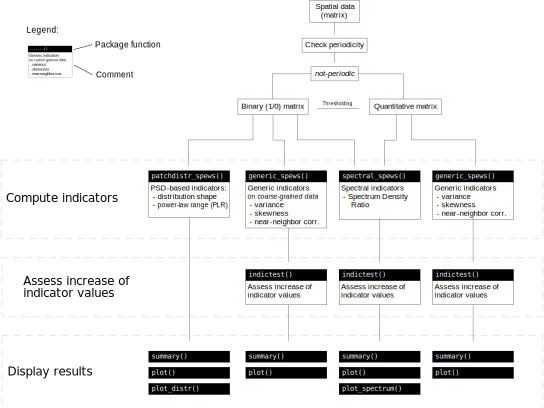
\includegraphics[width=1\textwidth]{./figures/flowchart.pdf}
  \caption{An EWS flowchart}
  \label{fig:flowchart}
\end{figure}

\section{Indicators for non-periodic patterns}

  \subsection{Generic indicators}

Any dynamical system approaching a transition point exhibits a phenomenon 
called Critical Slowing Down (CSD) \citep{kefi2013}. This means that for a given
perturbation, a system will take more time to recover when close to a threshold
than far from a threshold. As a result, it will depart further from its 
equilibrium (higher variance), have a stronger temporal autocorrelation and 
exhibit a higher skewness. Since these indicators only depend on simple 
properties of dynamical systems, they can, in principle, exist in many 
different systems, hence the adjective "Generic" \citep{scheffer2012}. 

This family of indicators can be computed using the \emph{generic\_spews} 
function. We work out an example below using data obtained from an ecological
model of forest gaps dynamics \citep{kubo1996}. This model is a cellular 
automaton with three parameters, $\alpha$, $\delta$ and $d$. 

The \emph{forestdat} dataset included with the package is the result of ten 
simulations with different values of $\delta$. It is a list of two components. 
The component \emph{parameters} is a data frame containing the parameters 
used for ten the simulations. The component \emph{matrices} is a list of 
ten boolean matrices representing a snapshot of the state of the cellular 
automaton around equilibrium (whether the cell is occupied by trees or not). 


\begin{Schunk}
\begin{Sinput}
R>   data(forestdat)
R>   str(matrices)
\end{Sinput}
\end{Schunk}

\begin{Schunk}
\begin{Soutput}
List of 10
 $ : logi [1:100, 1:100] TRUE TRUE TRUE TRUE TRUE TRUE ...
  ..- attr(*, "class")= chr [1:2] "binary_matrix" "matrix"
 $ : logi [1:100, 1:100] TRUE TRUE TRUE TRUE TRUE TRUE ...
  ..- attr(*, "class")= chr [1:2] "binary_matrix" "matrix"
[...]
  ..- attr(*, "class")= chr [1:2] "binary_matrix" "matrix"
 $ : logi [1:100, 1:100] FALSE TRUE TRUE TRUE FALSE FALSE ...
\end{Soutput}
\end{Schunk}

\begin{Schunk}
\begin{Sinput}
R>   head(forestdat$parameters)
\end{Sinput}
\begin{Soutput}
  simu alpha      delta    d
1    1   0.2 0.00000000 0.01
2    2   0.2 0.02222222 0.01
3    3   0.2 0.04444444 0.01
4    4   0.2 0.06666667 0.01
5    5   0.2 0.08888889 0.01
6    6   0.2 0.11111111 0.01
\end{Soutput}
\end{Schunk}

Given the parameters, the model is known to exhibit a transition for a value 
of delta close but superior to $0.2$. Let's compute the generic spatial 
indicators and display the result:
  
\begin{Schunk}
\begin{Sinput}
R>   gen_indic <- generic_spews(forestdat$matrices)
R>   summary(gen_indic)
\end{Sinput}
\begin{Soutput}
Generic Spatial Early-Warnings

 10 matrices (size: 100x100)

 Mat. #  Mean Moran's I Skewness Variance
      1 0.947   0.00265   -0.987  0.00340
      2 0.945   0.02904   -1.057  0.00348
      3 0.938   0.04076   -0.876  0.00389
      4 0.925   0.06376   -1.064  0.00577
      5 0.916   0.06873   -0.980  0.00636
      6 0.900   0.10533   -0.804  0.00725
      7 0.887   0.11271   -0.905  0.00955
      8 0.847   0.13693   -0.766  0.01265
      9 0.799   0.16556   -0.669  0.01779
     10 0.667   0.17228   -0.346  0.02616

Use as.data.frame() to retrieve values in a convenient form
\end{Soutput}
\end{Schunk}

The next step is to assess the significance of the indicator values. This is 
done by calling the \emph{indictest} generic: 
  
\begin{Schunk}
\begin{Sinput}
R>   gen_test <- indictest(gen_indic)
R>   print(gen_test)
\end{Sinput}
\begin{Soutput}
Generic Spatial Early-Warnings

 Mat. #  Mean Moran's I P>null     Skewness P>null     Variance
      1 0.947   0.00265  0.347       -0.987  0.539      0.00340
      2 0.945   0.02904  0.001 **    -1.057  0.792      0.00348
      3 0.938   0.04076  0.000 ***   -0.876  0.452      0.00389
      4 0.925   0.06376  0.000 ***   -1.064  0.986      0.00577
      5 0.916   0.06873  0.000 ***   -0.980  0.984      0.00636
      6 0.900   0.10533  0.000 ***   -0.804  0.926      0.00725
      7 0.887   0.11271  0.000 ***   -0.905  0.993      0.00955
      8 0.847   0.13693  0.000 ***   -0.766  0.997      0.01265
      9 0.799   0.16556  0.000 ***   -0.669  0.996      0.01779
     10 0.667   0.17228  0.000 ***   -0.346  0.964      0.02616
 P>null    
 0.0775 .  
 0.1110    
 0.1300    
 0.0000 ***
 0.0000 ***
 0.0000 ***
 0.0000 ***
 0.0000 ***
 0.0000 ***
 0.0000 ***

 Significance tested against 999 randomly shuffled matrices
 Signif. codes:  0 '***' 0.001 '**' 0.01 '*' 0.05 '.' 0.1 ' ' 1 
\end{Soutput}
\end{Schunk}

This object can then by plotted to display the indicator trends with the 
obtained null distribution: Fig. \ref{genindic_plot}. 
  
\begin{figure}
% Generate figure on the fly
  \includegraphics[width=1\textwidth]{./fig_genindic_plot.pdf}
  \caption{Generic indicator values for Kubo's forest-gap model. The line shows 
           the trend and the grey enveloppe the 5\% and 95\% quantiles of the 
           null distribution.}
  \label{genindic_plot}
\end{figure}

  \subsection{Spectral indicators}
  \label{spectral_ic}
  
  Because of the increased recovery time of a system approaching a tipping 
  point, neighbouring cells tend to be more like each other close to a tipping
  point. More geer
  
  
\begin{Schunk}
\begin{Sinput}
R>   data(forestdat)
R>   str(matrices)
\end{Sinput}
\end{Schunk}

\begin{Schunk}
\begin{Soutput}
List of 10
 $ : logi [1:100, 1:100] TRUE TRUE TRUE TRUE TRUE TRUE ...
  ..- attr(*, "class")= chr [1:2] "binary_matrix" "matrix"
 $ : logi [1:100, 1:100] TRUE TRUE TRUE TRUE TRUE TRUE ...
  ..- attr(*, "class")= chr [1:2] "binary_matrix" "matrix"
[...]
  ..- attr(*, "class")= chr [1:2] "binary_matrix" "matrix"
 $ : logi [1:100, 1:100] FALSE TRUE TRUE TRUE FALSE FALSE ...
\end{Soutput}
\end{Schunk}

\begin{Schunk}
\begin{Sinput}
R>   head(forestdat$parameters)
\end{Sinput}
\begin{Soutput}
  simu alpha      delta    d
1    1   0.2 0.00000000 0.01
2    2   0.2 0.02222222 0.01
3    3   0.2 0.04444444 0.01
4    4   0.2 0.06666667 0.01
5    5   0.2 0.08888889 0.01
6    6   0.2 0.11111111 0.01
\end{Soutput}
\end{Schunk}

  \subsection{Patch-based indicators}

% Task function: give shape of distribution + percolation points of each

% fitpsd





\section{Using the package: additional remarks}



  \subsection{Leveraging plyr's abilities} 
  
    \subsubsection{Progress report}
    
    \subsubsection{Parallel processing}
    
    
\section*{Acknowledgments}

\section*{References}

\bibliographystyle{apa}
\bibliography{refs}

\end{document}
